
%% Style 54

\cxset{appendix name/.store in=\appendix@cx}
\cxset{
 name=,
 numbering=arabic,
 number font-size=\Large,
 number before={},
 number after=,
 number dot=,
 number position=rightname,
 number color=\color{blue},
 chapter color={blue},
 chapter font-size=\Large,
 chapter before=\par\hfill\hfill,
 chapter after=\hfill,
 title font-family=\rmfamily,
 title font-color=\color{blue},
 title font-weight=,
 title font-size=\LARGE,
 title beforeskip=\hfill,
 title afterskip={\vspace*{20pt}},
 header style=empty}
\chapter{{STYLE FIFTY FOUR}}


This is an unusual book with a rather unique style. The vertical rule is simple and breaks the monotony of a book that is heavy on text.\index{rules!style 54}

\begin{figure}[ht]
\fbox{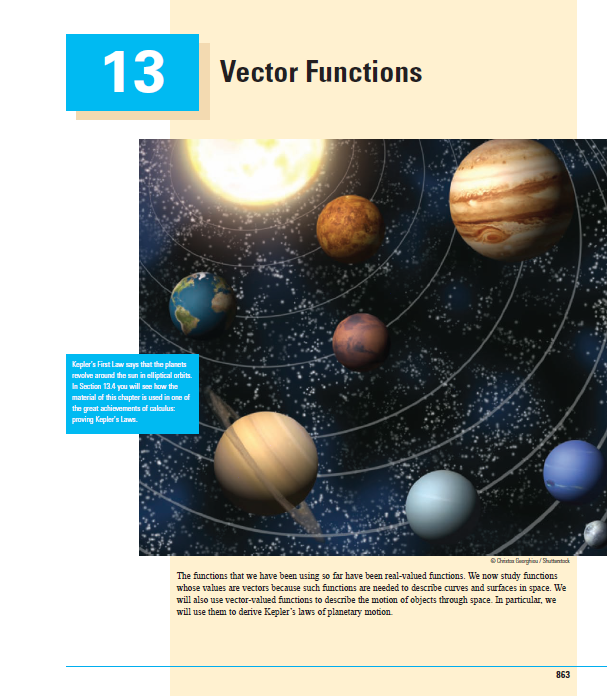
\includegraphics[width=0.48\textwidth]{./chapters/chapter54}}\hfill
\fbox{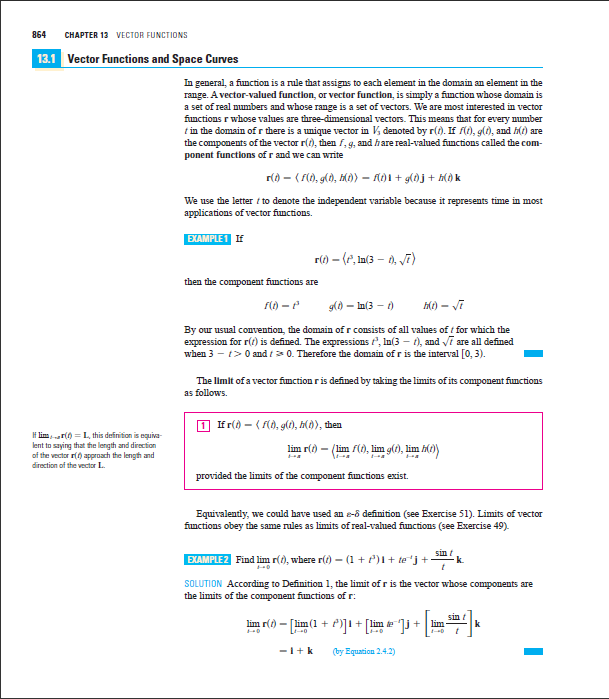
\includegraphics[width=0.48\textwidth]{./chapters/chapter54a}}
\caption{Style 54 from Steward's Calculus.}
\end{figure}
